% Created by tikzDevice version 0.10.1 on 2018-01-15 11:46:38
% !TEX encoding = UTF-8 Unicode
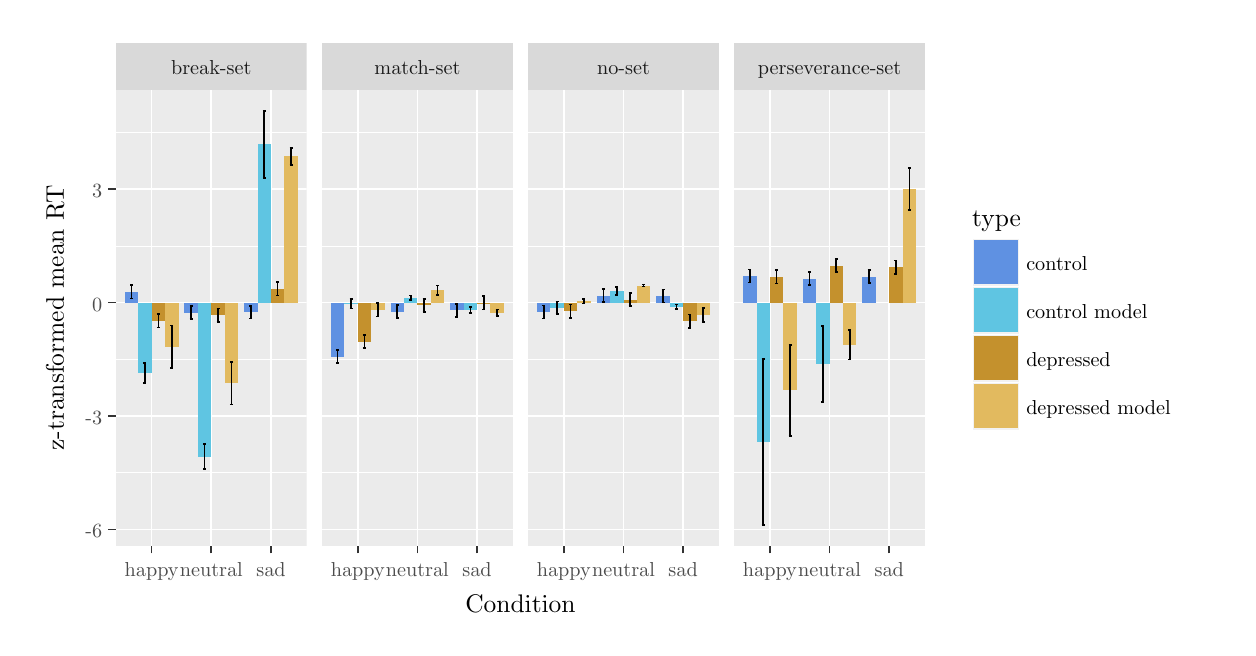
\begin{tikzpicture}[x=1pt,y=1pt]
\definecolor{fillColor}{RGB}{255,255,255}
\path[use as bounding box,fill=fillColor,fill opacity=0.00] (0,0) rectangle (433.62,216.81);
\begin{scope}
\path[clip] (  0.00,  0.00) rectangle (433.62,216.81);
\definecolor{drawColor}{RGB}{255,255,255}
\definecolor{fillColor}{RGB}{255,255,255}

\path[draw=drawColor,line width= 0.6pt,line join=round,line cap=round,fill=fillColor] (  0.00,  0.00) rectangle (433.62,216.81);
\end{scope}
\begin{scope}
\path[clip] ( 31.87, 29.59) rectangle (100.84,194.25);
\definecolor{fillColor}{gray}{0.92}

\path[fill=fillColor] ( 31.87, 29.59) rectangle (100.84,194.25);
\definecolor{drawColor}{RGB}{255,255,255}

\path[draw=drawColor,line width= 0.3pt,line join=round] ( 31.87, 55.96) --
	(100.84, 55.96);

\path[draw=drawColor,line width= 0.3pt,line join=round] ( 31.87, 96.94) --
	(100.84, 96.94);

\path[draw=drawColor,line width= 0.3pt,line join=round] ( 31.87,137.93) --
	(100.84,137.93);

\path[draw=drawColor,line width= 0.3pt,line join=round] ( 31.87,178.91) --
	(100.84,178.91);

\path[draw=drawColor,line width= 0.6pt,line join=round] ( 31.87, 35.47) --
	(100.84, 35.47);

\path[draw=drawColor,line width= 0.6pt,line join=round] ( 31.87, 76.45) --
	(100.84, 76.45);

\path[draw=drawColor,line width= 0.6pt,line join=round] ( 31.87,117.44) --
	(100.84,117.44);

\path[draw=drawColor,line width= 0.6pt,line join=round] ( 31.87,158.42) --
	(100.84,158.42);

\path[draw=drawColor,line width= 0.6pt,line join=round] ( 44.80, 29.59) --
	( 44.80,194.25);

\path[draw=drawColor,line width= 0.6pt,line join=round] ( 66.36, 29.59) --
	( 66.36,194.25);

\path[draw=drawColor,line width= 0.6pt,line join=round] ( 87.91, 29.59) --
	( 87.91,194.25);
\definecolor{fillColor}{RGB}{226,186,95}

\path[fill=fillColor] ( 49.65,101.49) rectangle ( 54.50,117.44);
\definecolor{fillColor}{RGB}{196,145,45}

\path[fill=fillColor] ( 44.80,110.85) rectangle ( 49.65,117.44);
\definecolor{fillColor}{RGB}{95,197,226}

\path[fill=fillColor] ( 39.95, 92.05) rectangle ( 44.80,117.44);
\definecolor{fillColor}{RGB}{95,145,226}

\path[fill=fillColor] ( 35.10,117.44) rectangle ( 39.95,121.36);
\definecolor{fillColor}{RGB}{226,186,95}

\path[fill=fillColor] ( 71.21, 88.35) rectangle ( 76.06,117.44);
\definecolor{fillColor}{RGB}{196,145,45}

\path[fill=fillColor] ( 66.36,112.93) rectangle ( 71.21,117.44);
\definecolor{fillColor}{RGB}{95,197,226}

\path[fill=fillColor] ( 61.51, 61.85) rectangle ( 66.36,117.44);
\definecolor{fillColor}{RGB}{95,145,226}

\path[fill=fillColor] ( 56.66,113.84) rectangle ( 61.51,117.44);
\definecolor{fillColor}{RGB}{226,186,95}

\path[fill=fillColor] ( 92.76,117.44) rectangle ( 97.61,170.30);
\definecolor{fillColor}{RGB}{196,145,45}

\path[fill=fillColor] ( 87.91,117.44) rectangle ( 92.76,122.50);
\definecolor{fillColor}{RGB}{95,197,226}

\path[fill=fillColor] ( 83.06,117.44) rectangle ( 87.91,174.63);
\definecolor{fillColor}{RGB}{95,145,226}

\path[fill=fillColor] ( 78.21,114.00) rectangle ( 83.06,117.44);
\definecolor{drawColor}{RGB}{0,0,0}

\path[draw=drawColor,line width= 0.6pt,line join=round] ( 51.54,109.16) --
	( 52.62,109.16);

\path[draw=drawColor,line width= 0.6pt,line join=round] ( 52.08,109.16) --
	( 52.08, 93.83);

\path[draw=drawColor,line width= 0.6pt,line join=round] ( 51.54, 93.83) --
	( 52.62, 93.83);

\path[draw=drawColor,line width= 0.6pt,line join=round] ( 46.69,113.27) --
	( 47.77,113.27);

\path[draw=drawColor,line width= 0.6pt,line join=round] ( 47.23,113.27) --
	( 47.23,108.42);

\path[draw=drawColor,line width= 0.6pt,line join=round] ( 46.69,108.42) --
	( 47.77,108.42);

\path[draw=drawColor,line width= 0.6pt,line join=round] ( 41.84, 95.62) --
	( 42.92, 95.62);

\path[draw=drawColor,line width= 0.6pt,line join=round] ( 42.38, 95.62) --
	( 42.38, 88.49);

\path[draw=drawColor,line width= 0.6pt,line join=round] ( 41.84, 88.49) --
	( 42.92, 88.49);

\path[draw=drawColor,line width= 0.6pt,line join=round] ( 36.99,123.75) --
	( 38.07,123.75);

\path[draw=drawColor,line width= 0.6pt,line join=round] ( 37.53,123.75) --
	( 37.53,118.96);

\path[draw=drawColor,line width= 0.6pt,line join=round] ( 36.99,118.96) --
	( 38.07,118.96);

\path[draw=drawColor,line width= 0.6pt,line join=round] ( 73.09, 96.11) --
	( 74.17, 96.11);

\path[draw=drawColor,line width= 0.6pt,line join=round] ( 73.63, 96.11) --
	( 73.63, 80.59);

\path[draw=drawColor,line width= 0.6pt,line join=round] ( 73.09, 80.59) --
	( 74.17, 80.59);

\path[draw=drawColor,line width= 0.6pt,line join=round] ( 68.24,115.34) --
	( 69.32,115.34);

\path[draw=drawColor,line width= 0.6pt,line join=round] ( 68.78,115.34) --
	( 68.78,110.51);

\path[draw=drawColor,line width= 0.6pt,line join=round] ( 68.24,110.51) --
	( 69.32,110.51);

\path[draw=drawColor,line width= 0.6pt,line join=round] ( 63.39, 66.38) --
	( 64.47, 66.38);

\path[draw=drawColor,line width= 0.6pt,line join=round] ( 63.93, 66.38) --
	( 63.93, 57.33);

\path[draw=drawColor,line width= 0.6pt,line join=round] ( 63.39, 57.33) --
	( 64.47, 57.33);

\path[draw=drawColor,line width= 0.6pt,line join=round] ( 58.54,116.17) --
	( 59.62,116.17);

\path[draw=drawColor,line width= 0.6pt,line join=round] ( 59.08,116.17) --
	( 59.08,111.51);

\path[draw=drawColor,line width= 0.6pt,line join=round] ( 58.54,111.51) --
	( 59.62,111.51);

\path[draw=drawColor,line width= 0.6pt,line join=round] ( 94.65,173.32) --
	( 95.72,173.32);

\path[draw=drawColor,line width= 0.6pt,line join=round] ( 95.18,173.32) --
	( 95.18,167.28);

\path[draw=drawColor,line width= 0.6pt,line join=round] ( 94.65,167.28) --
	( 95.72,167.28);

\path[draw=drawColor,line width= 0.6pt,line join=round] ( 89.80,124.93) --
	( 90.87,124.93);

\path[draw=drawColor,line width= 0.6pt,line join=round] ( 90.33,124.93) --
	( 90.33,120.08);

\path[draw=drawColor,line width= 0.6pt,line join=round] ( 89.80,120.08) --
	( 90.87,120.08);

\path[draw=drawColor,line width= 0.6pt,line join=round] ( 84.95,186.76) --
	( 86.02,186.76);

\path[draw=drawColor,line width= 0.6pt,line join=round] ( 85.48,186.76) --
	( 85.48,162.50);

\path[draw=drawColor,line width= 0.6pt,line join=round] ( 84.95,162.50) --
	( 86.02,162.50);

\path[draw=drawColor,line width= 0.6pt,line join=round] ( 80.10,116.33) --
	( 81.17,116.33);

\path[draw=drawColor,line width= 0.6pt,line join=round] ( 80.64,116.33) --
	( 80.64,111.66);

\path[draw=drawColor,line width= 0.6pt,line join=round] ( 80.10,111.66) --
	( 81.17,111.66);
\end{scope}
\begin{scope}
\path[clip] (106.34, 29.59) rectangle (175.31,194.25);
\definecolor{fillColor}{gray}{0.92}

\path[fill=fillColor] (106.34, 29.59) rectangle (175.31,194.25);
\definecolor{drawColor}{RGB}{255,255,255}

\path[draw=drawColor,line width= 0.3pt,line join=round] (106.34, 55.96) --
	(175.31, 55.96);

\path[draw=drawColor,line width= 0.3pt,line join=round] (106.34, 96.94) --
	(175.31, 96.94);

\path[draw=drawColor,line width= 0.3pt,line join=round] (106.34,137.93) --
	(175.31,137.93);

\path[draw=drawColor,line width= 0.3pt,line join=round] (106.34,178.91) --
	(175.31,178.91);

\path[draw=drawColor,line width= 0.6pt,line join=round] (106.34, 35.47) --
	(175.31, 35.47);

\path[draw=drawColor,line width= 0.6pt,line join=round] (106.34, 76.45) --
	(175.31, 76.45);

\path[draw=drawColor,line width= 0.6pt,line join=round] (106.34,117.44) --
	(175.31,117.44);

\path[draw=drawColor,line width= 0.6pt,line join=round] (106.34,158.42) --
	(175.31,158.42);

\path[draw=drawColor,line width= 0.6pt,line join=round] (119.27, 29.59) --
	(119.27,194.25);

\path[draw=drawColor,line width= 0.6pt,line join=round] (140.83, 29.59) --
	(140.83,194.25);

\path[draw=drawColor,line width= 0.6pt,line join=round] (162.38, 29.59) --
	(162.38,194.25);
\definecolor{fillColor}{RGB}{226,186,95}

\path[fill=fillColor] (124.12,114.88) rectangle (128.97,117.44);
\definecolor{fillColor}{RGB}{196,145,45}

\path[fill=fillColor] (119.27,103.36) rectangle (124.12,117.44);
\definecolor{fillColor}{RGB}{95,197,226}

\path[fill=fillColor] (114.42,117.05) rectangle (119.27,117.44);
\definecolor{fillColor}{RGB}{95,145,226}

\path[fill=fillColor] (109.57, 97.92) rectangle (114.42,117.44);
\definecolor{fillColor}{RGB}{226,186,95}

\path[fill=fillColor] (145.68,117.44) rectangle (150.53,121.90);
\definecolor{fillColor}{RGB}{196,145,45}

\path[fill=fillColor] (140.83,116.44) rectangle (145.68,117.44);
\definecolor{fillColor}{RGB}{95,197,226}

\path[fill=fillColor] (135.98,117.44) rectangle (140.83,119.20);
\definecolor{fillColor}{RGB}{95,145,226}

\path[fill=fillColor] (131.13,114.17) rectangle (135.98,117.44);
\definecolor{fillColor}{RGB}{226,186,95}

\path[fill=fillColor] (167.23,113.82) rectangle (172.08,117.44);
\definecolor{fillColor}{RGB}{196,145,45}

\path[fill=fillColor] (162.38,117.39) rectangle (167.23,117.44);
\definecolor{fillColor}{RGB}{95,197,226}

\path[fill=fillColor] (157.53,114.81) rectangle (162.38,117.44);
\definecolor{fillColor}{RGB}{95,145,226}

\path[fill=fillColor] (152.68,114.61) rectangle (157.53,117.44);
\definecolor{drawColor}{RGB}{0,0,0}

\path[draw=drawColor,line width= 0.6pt,line join=round] (126.01,117.35) --
	(127.09,117.35);

\path[draw=drawColor,line width= 0.6pt,line join=round] (126.55,117.35) --
	(126.55,112.41);

\path[draw=drawColor,line width= 0.6pt,line join=round] (126.01,112.41) --
	(127.09,112.41);

\path[draw=drawColor,line width= 0.6pt,line join=round] (121.16,105.78) --
	(122.24,105.78);

\path[draw=drawColor,line width= 0.6pt,line join=round] (121.70,105.78) --
	(121.70,100.94);

\path[draw=drawColor,line width= 0.6pt,line join=round] (121.16,100.94) --
	(122.24,100.94);

\path[draw=drawColor,line width= 0.6pt,line join=round] (116.31,118.75) --
	(117.39,118.75);

\path[draw=drawColor,line width= 0.6pt,line join=round] (116.85,118.75) --
	(116.85,115.34);

\path[draw=drawColor,line width= 0.6pt,line join=round] (116.31,115.34) --
	(117.39,115.34);

\path[draw=drawColor,line width= 0.6pt,line join=round] (111.46,100.26) --
	(112.54,100.26);

\path[draw=drawColor,line width= 0.6pt,line join=round] (112.00,100.26) --
	(112.00, 95.58);

\path[draw=drawColor,line width= 0.6pt,line join=round] (111.46, 95.58) --
	(112.54, 95.58);

\path[draw=drawColor,line width= 0.6pt,line join=round] (147.56,123.59) --
	(148.64,123.59);

\path[draw=drawColor,line width= 0.6pt,line join=round] (148.10,123.59) --
	(148.10,120.21);

\path[draw=drawColor,line width= 0.6pt,line join=round] (147.56,120.21) --
	(148.64,120.21);

\path[draw=drawColor,line width= 0.6pt,line join=round] (142.71,118.86) --
	(143.79,118.86);

\path[draw=drawColor,line width= 0.6pt,line join=round] (143.25,118.86) --
	(143.25,114.03);

\path[draw=drawColor,line width= 0.6pt,line join=round] (142.71,114.03) --
	(143.79,114.03);

\path[draw=drawColor,line width= 0.6pt,line join=round] (137.86,119.99) --
	(138.94,119.99);

\path[draw=drawColor,line width= 0.6pt,line join=round] (138.40,119.99) --
	(138.40,118.41);

\path[draw=drawColor,line width= 0.6pt,line join=round] (137.86,118.41) --
	(138.94,118.41);

\path[draw=drawColor,line width= 0.6pt,line join=round] (133.01,116.50) --
	(134.09,116.50);

\path[draw=drawColor,line width= 0.6pt,line join=round] (133.55,116.50) --
	(133.55,111.83);

\path[draw=drawColor,line width= 0.6pt,line join=round] (133.01,111.83) --
	(134.09,111.83);

\path[draw=drawColor,line width= 0.6pt,line join=round] (169.12,115.01) --
	(170.19,115.01);

\path[draw=drawColor,line width= 0.6pt,line join=round] (169.65,115.01) --
	(169.65,112.64);

\path[draw=drawColor,line width= 0.6pt,line join=round] (169.12,112.64) --
	(170.19,112.64);

\path[draw=drawColor,line width= 0.6pt,line join=round] (164.27,119.81) --
	(165.34,119.81);

\path[draw=drawColor,line width= 0.6pt,line join=round] (164.80,119.81) --
	(164.80,114.97);

\path[draw=drawColor,line width= 0.6pt,line join=round] (164.27,114.97) --
	(165.34,114.97);

\path[draw=drawColor,line width= 0.6pt,line join=round] (159.42,115.81) --
	(160.49,115.81);

\path[draw=drawColor,line width= 0.6pt,line join=round] (159.96,115.81) --
	(159.96,113.82);

\path[draw=drawColor,line width= 0.6pt,line join=round] (159.42,113.82) --
	(160.49,113.82);

\path[draw=drawColor,line width= 0.6pt,line join=round] (154.57,116.95) --
	(155.64,116.95);

\path[draw=drawColor,line width= 0.6pt,line join=round] (155.11,116.95) --
	(155.11,112.28);

\path[draw=drawColor,line width= 0.6pt,line join=round] (154.57,112.28) --
	(155.64,112.28);
\end{scope}
\begin{scope}
\path[clip] (180.81, 29.59) rectangle (249.78,194.25);
\definecolor{fillColor}{gray}{0.92}

\path[fill=fillColor] (180.81, 29.59) rectangle (249.78,194.25);
\definecolor{drawColor}{RGB}{255,255,255}

\path[draw=drawColor,line width= 0.3pt,line join=round] (180.81, 55.96) --
	(249.78, 55.96);

\path[draw=drawColor,line width= 0.3pt,line join=round] (180.81, 96.94) --
	(249.78, 96.94);

\path[draw=drawColor,line width= 0.3pt,line join=round] (180.81,137.93) --
	(249.78,137.93);

\path[draw=drawColor,line width= 0.3pt,line join=round] (180.81,178.91) --
	(249.78,178.91);

\path[draw=drawColor,line width= 0.6pt,line join=round] (180.81, 35.47) --
	(249.78, 35.47);

\path[draw=drawColor,line width= 0.6pt,line join=round] (180.81, 76.45) --
	(249.78, 76.45);

\path[draw=drawColor,line width= 0.6pt,line join=round] (180.81,117.44) --
	(249.78,117.44);

\path[draw=drawColor,line width= 0.6pt,line join=round] (180.81,158.42) --
	(249.78,158.42);

\path[draw=drawColor,line width= 0.6pt,line join=round] (193.74, 29.59) --
	(193.74,194.25);

\path[draw=drawColor,line width= 0.6pt,line join=round] (215.30, 29.59) --
	(215.30,194.25);

\path[draw=drawColor,line width= 0.6pt,line join=round] (236.85, 29.59) --
	(236.85,194.25);
\definecolor{fillColor}{RGB}{226,186,95}

\path[fill=fillColor] (198.59,117.44) rectangle (203.44,117.94);
\definecolor{fillColor}{RGB}{196,145,45}

\path[fill=fillColor] (193.74,114.40) rectangle (198.59,117.44);
\definecolor{fillColor}{RGB}{95,197,226}

\path[fill=fillColor] (188.89,115.54) rectangle (193.74,117.44);
\definecolor{fillColor}{RGB}{95,145,226}

\path[fill=fillColor] (184.05,114.04) rectangle (188.89,117.44);
\definecolor{fillColor}{RGB}{226,186,95}

\path[fill=fillColor] (220.15,117.44) rectangle (225.00,123.64);
\definecolor{fillColor}{RGB}{196,145,45}

\path[fill=fillColor] (215.30,117.44) rectangle (220.15,118.58);
\definecolor{fillColor}{RGB}{95,197,226}

\path[fill=fillColor] (210.45,117.44) rectangle (215.30,121.71);
\definecolor{fillColor}{RGB}{95,145,226}

\path[fill=fillColor] (205.60,117.44) rectangle (210.45,120.01);
\definecolor{fillColor}{RGB}{226,186,95}

\path[fill=fillColor] (241.70,112.95) rectangle (246.55,117.44);
\definecolor{fillColor}{RGB}{196,145,45}

\path[fill=fillColor] (236.85,110.80) rectangle (241.70,117.44);
\definecolor{fillColor}{RGB}{95,197,226}

\path[fill=fillColor] (232.00,115.97) rectangle (236.85,117.44);
\definecolor{fillColor}{RGB}{95,145,226}

\path[fill=fillColor] (227.15,117.44) rectangle (232.00,119.81);
\definecolor{drawColor}{RGB}{0,0,0}

\path[draw=drawColor,line width= 0.6pt,line join=round] (200.48,118.71) --
	(201.56,118.71);

\path[draw=drawColor,line width= 0.6pt,line join=round] (201.02,118.71) --
	(201.02,117.18);

\path[draw=drawColor,line width= 0.6pt,line join=round] (200.48,117.18) --
	(201.56,117.18);

\path[draw=drawColor,line width= 0.6pt,line join=round] (195.63,116.82) --
	(196.71,116.82);

\path[draw=drawColor,line width= 0.6pt,line join=round] (196.17,116.82) --
	(196.17,111.98);

\path[draw=drawColor,line width= 0.6pt,line join=round] (195.63,111.98) --
	(196.71,111.98);

\path[draw=drawColor,line width= 0.6pt,line join=round] (190.78,117.81) --
	(191.86,117.81);

\path[draw=drawColor,line width= 0.6pt,line join=round] (191.32,117.81) --
	(191.32,113.27);

\path[draw=drawColor,line width= 0.6pt,line join=round] (190.78,113.27) --
	(191.86,113.27);

\path[draw=drawColor,line width= 0.6pt,line join=round] (185.93,116.38) --
	(187.01,116.38);

\path[draw=drawColor,line width= 0.6pt,line join=round] (186.47,116.38) --
	(186.47,111.70);

\path[draw=drawColor,line width= 0.6pt,line join=round] (185.93,111.70) --
	(187.01,111.70);

\path[draw=drawColor,line width= 0.6pt,line join=round] (222.03,124.00) --
	(223.11,124.00);

\path[draw=drawColor,line width= 0.6pt,line join=round] (222.57,124.00) --
	(222.57,123.27);

\path[draw=drawColor,line width= 0.6pt,line join=round] (222.03,123.27) --
	(223.11,123.27);

\path[draw=drawColor,line width= 0.6pt,line join=round] (217.18,121.01) --
	(218.26,121.01);

\path[draw=drawColor,line width= 0.6pt,line join=round] (217.72,121.01) --
	(217.72,116.16);

\path[draw=drawColor,line width= 0.6pt,line join=round] (217.18,116.16) --
	(218.26,116.16);

\path[draw=drawColor,line width= 0.6pt,line join=round] (212.33,123.15) --
	(213.41,123.15);

\path[draw=drawColor,line width= 0.6pt,line join=round] (212.87,123.15) --
	(212.87,120.26);

\path[draw=drawColor,line width= 0.6pt,line join=round] (212.33,120.26) --
	(213.41,120.26);

\path[draw=drawColor,line width= 0.6pt,line join=round] (207.48,122.34) --
	(208.56,122.34);

\path[draw=drawColor,line width= 0.6pt,line join=round] (208.02,122.34) --
	(208.02,117.68);

\path[draw=drawColor,line width= 0.6pt,line join=round] (207.48,117.68) --
	(208.56,117.68);

\path[draw=drawColor,line width= 0.6pt,line join=round] (243.59,115.46) --
	(244.66,115.46);

\path[draw=drawColor,line width= 0.6pt,line join=round] (244.12,115.46) --
	(244.12,110.44);

\path[draw=drawColor,line width= 0.6pt,line join=round] (243.59,110.44) --
	(244.66,110.44);

\path[draw=drawColor,line width= 0.6pt,line join=round] (238.74,113.22) --
	(239.81,113.22);

\path[draw=drawColor,line width= 0.6pt,line join=round] (239.28,113.22) --
	(239.28,108.38);

\path[draw=drawColor,line width= 0.6pt,line join=round] (238.74,108.38) --
	(239.81,108.38);

\path[draw=drawColor,line width= 0.6pt,line join=round] (233.89,116.83) --
	(234.96,116.83);

\path[draw=drawColor,line width= 0.6pt,line join=round] (234.43,116.83) --
	(234.43,115.11);

\path[draw=drawColor,line width= 0.6pt,line join=round] (233.89,115.11) --
	(234.96,115.11);

\path[draw=drawColor,line width= 0.6pt,line join=round] (229.04,122.14) --
	(230.12,122.14);

\path[draw=drawColor,line width= 0.6pt,line join=round] (229.58,122.14) --
	(229.58,117.47);

\path[draw=drawColor,line width= 0.6pt,line join=round] (229.04,117.47) --
	(230.12,117.47);
\end{scope}
\begin{scope}
\path[clip] (255.28, 29.59) rectangle (324.25,194.25);
\definecolor{fillColor}{gray}{0.92}

\path[fill=fillColor] (255.28, 29.59) rectangle (324.25,194.25);
\definecolor{drawColor}{RGB}{255,255,255}

\path[draw=drawColor,line width= 0.3pt,line join=round] (255.28, 55.96) --
	(324.25, 55.96);

\path[draw=drawColor,line width= 0.3pt,line join=round] (255.28, 96.94) --
	(324.25, 96.94);

\path[draw=drawColor,line width= 0.3pt,line join=round] (255.28,137.93) --
	(324.25,137.93);

\path[draw=drawColor,line width= 0.3pt,line join=round] (255.28,178.91) --
	(324.25,178.91);

\path[draw=drawColor,line width= 0.6pt,line join=round] (255.28, 35.47) --
	(324.25, 35.47);

\path[draw=drawColor,line width= 0.6pt,line join=round] (255.28, 76.45) --
	(324.25, 76.45);

\path[draw=drawColor,line width= 0.6pt,line join=round] (255.28,117.44) --
	(324.25,117.44);

\path[draw=drawColor,line width= 0.6pt,line join=round] (255.28,158.42) --
	(324.25,158.42);

\path[draw=drawColor,line width= 0.6pt,line join=round] (268.21, 29.59) --
	(268.21,194.25);

\path[draw=drawColor,line width= 0.6pt,line join=round] (289.77, 29.59) --
	(289.77,194.25);

\path[draw=drawColor,line width= 0.6pt,line join=round] (311.32, 29.59) --
	(311.32,194.25);
\definecolor{fillColor}{RGB}{226,186,95}

\path[fill=fillColor] (273.06, 85.75) rectangle (277.91,117.44);
\definecolor{fillColor}{RGB}{196,145,45}

\path[fill=fillColor] (268.21,117.44) rectangle (273.06,126.75);
\definecolor{fillColor}{RGB}{95,197,226}

\path[fill=fillColor] (263.37, 67.13) rectangle (268.21,117.44);
\definecolor{fillColor}{RGB}{95,145,226}

\path[fill=fillColor] (258.52,117.44) rectangle (263.37,127.04);
\definecolor{fillColor}{RGB}{226,186,95}

\path[fill=fillColor] (294.62,102.22) rectangle (299.47,117.44);
\definecolor{fillColor}{RGB}{196,145,45}

\path[fill=fillColor] (289.77,117.44) rectangle (294.62,130.84);
\definecolor{fillColor}{RGB}{95,197,226}

\path[fill=fillColor] (284.92, 95.38) rectangle (289.77,117.44);
\definecolor{fillColor}{RGB}{95,145,226}

\path[fill=fillColor] (280.07,117.44) rectangle (284.92,126.10);
\definecolor{fillColor}{RGB}{226,186,95}

\path[fill=fillColor] (316.17,117.44) rectangle (321.02,158.47);
\definecolor{fillColor}{RGB}{196,145,45}

\path[fill=fillColor] (311.32,117.44) rectangle (316.17,130.32);
\definecolor{fillColor}{RGB}{95,145,226}

\path[fill=fillColor] (301.62,117.44) rectangle (306.47,126.87);
\definecolor{drawColor}{RGB}{0,0,0}

\path[draw=drawColor,line width= 0.6pt,line join=round] (274.95,102.21) --
	(276.03,102.21);

\path[draw=drawColor,line width= 0.6pt,line join=round] (275.49,102.21) --
	(275.49, 69.30);

\path[draw=drawColor,line width= 0.6pt,line join=round] (274.95, 69.30) --
	(276.03, 69.30);

\path[draw=drawColor,line width= 0.6pt,line join=round] (270.10,129.17) --
	(271.18,129.17);

\path[draw=drawColor,line width= 0.6pt,line join=round] (270.64,129.17) --
	(270.64,124.33);

\path[draw=drawColor,line width= 0.6pt,line join=round] (270.10,124.33) --
	(271.18,124.33);

\path[draw=drawColor,line width= 0.6pt,line join=round] (265.25, 97.19) --
	(266.33, 97.19);

\path[draw=drawColor,line width= 0.6pt,line join=round] (265.79, 97.19) --
	(265.79, 37.07);

\path[draw=drawColor,line width= 0.6pt,line join=round] (265.25, 37.07) --
	(266.33, 37.07);

\path[draw=drawColor,line width= 0.6pt,line join=round] (260.40,129.38) --
	(261.48,129.38);

\path[draw=drawColor,line width= 0.6pt,line join=round] (260.94,129.38) --
	(260.94,124.71);

\path[draw=drawColor,line width= 0.6pt,line join=round] (260.40,124.71) --
	(261.48,124.71);

\path[draw=drawColor,line width= 0.6pt,line join=round] (296.50,107.52) --
	(297.58,107.52);

\path[draw=drawColor,line width= 0.6pt,line join=round] (297.04,107.52) --
	(297.04, 96.92);

\path[draw=drawColor,line width= 0.6pt,line join=round] (296.50, 96.92) --
	(297.58, 96.92);

\path[draw=drawColor,line width= 0.6pt,line join=round] (291.65,133.26) --
	(292.73,133.26);

\path[draw=drawColor,line width= 0.6pt,line join=round] (292.19,133.26) --
	(292.19,128.42);

\path[draw=drawColor,line width= 0.6pt,line join=round] (291.65,128.42) --
	(292.73,128.42);

\path[draw=drawColor,line width= 0.6pt,line join=round] (286.80,109.10) --
	(287.88,109.10);

\path[draw=drawColor,line width= 0.6pt,line join=round] (287.34,109.10) --
	(287.34, 81.66);

\path[draw=drawColor,line width= 0.6pt,line join=round] (286.80, 81.66) --
	(287.88, 81.66);

\path[draw=drawColor,line width= 0.6pt,line join=round] (281.95,128.43) --
	(283.03,128.43);

\path[draw=drawColor,line width= 0.6pt,line join=round] (282.49,128.43) --
	(282.49,123.77);

\path[draw=drawColor,line width= 0.6pt,line join=round] (281.95,123.77) --
	(283.03,123.77);

\path[draw=drawColor,line width= 0.6pt,line join=round] (318.06,166.13) --
	(319.13,166.13);

\path[draw=drawColor,line width= 0.6pt,line join=round] (318.60,166.13) --
	(318.60,150.81);

\path[draw=drawColor,line width= 0.6pt,line join=round] (318.06,150.81) --
	(319.13,150.81);

\path[draw=drawColor,line width= 0.6pt,line join=round] (313.21,132.73) --
	(314.28,132.73);

\path[draw=drawColor,line width= 0.6pt,line join=round] (313.75,132.73) --
	(313.75,127.90);

\path[draw=drawColor,line width= 0.6pt,line join=round] (313.21,127.90) --
	(314.28,127.90);

\path[draw=drawColor,line width= 0.6pt,line join=round] (303.51,129.21) --
	(304.59,129.21);

\path[draw=drawColor,line width= 0.6pt,line join=round] (304.05,129.21) --
	(304.05,124.54);

\path[draw=drawColor,line width= 0.6pt,line join=round] (303.51,124.54) --
	(304.59,124.54);
\end{scope}
\begin{scope}
\path[clip] ( 31.87,194.25) rectangle (100.84,211.31);
\definecolor{fillColor}{gray}{0.85}

\path[fill=fillColor] ( 31.87,194.25) rectangle (100.84,211.31);
\definecolor{drawColor}{gray}{0.10}

\node[text=drawColor,anchor=base,inner sep=0pt, outer sep=0pt, scale=  0.73] at ( 66.36,199.75) {break-set};
\end{scope}
\begin{scope}
\path[clip] (106.34,194.25) rectangle (175.31,211.31);
\definecolor{fillColor}{gray}{0.85}

\path[fill=fillColor] (106.34,194.25) rectangle (175.31,211.31);
\definecolor{drawColor}{gray}{0.10}

\node[text=drawColor,anchor=base,inner sep=0pt, outer sep=0pt, scale=  0.73] at (140.83,199.75) {match-set};
\end{scope}
\begin{scope}
\path[clip] (180.81,194.25) rectangle (249.78,211.31);
\definecolor{fillColor}{gray}{0.85}

\path[fill=fillColor] (180.81,194.25) rectangle (249.78,211.31);
\definecolor{drawColor}{gray}{0.10}

\node[text=drawColor,anchor=base,inner sep=0pt, outer sep=0pt, scale=  0.73] at (215.30,199.75) {no-set};
\end{scope}
\begin{scope}
\path[clip] (255.28,194.25) rectangle (324.25,211.31);
\definecolor{fillColor}{gray}{0.85}

\path[fill=fillColor] (255.28,194.25) rectangle (324.25,211.31);
\definecolor{drawColor}{gray}{0.10}

\node[text=drawColor,anchor=base,inner sep=0pt, outer sep=0pt, scale=  0.73] at (289.77,199.75) {perseverance-set};
\end{scope}
\begin{scope}
\path[clip] (  0.00,  0.00) rectangle (433.62,216.81);
\definecolor{drawColor}{gray}{0.20}

\path[draw=drawColor,line width= 0.6pt,line join=round] ( 44.80, 26.84) --
	( 44.80, 29.59);

\path[draw=drawColor,line width= 0.6pt,line join=round] ( 66.36, 26.84) --
	( 66.36, 29.59);

\path[draw=drawColor,line width= 0.6pt,line join=round] ( 87.91, 26.84) --
	( 87.91, 29.59);
\end{scope}
\begin{scope}
\path[clip] (  0.00,  0.00) rectangle (433.62,216.81);
\definecolor{drawColor}{gray}{0.30}

\node[text=drawColor,anchor=base,inner sep=0pt, outer sep=0pt, scale=  0.73] at ( 44.80, 18.58) {happy};

\node[text=drawColor,anchor=base,inner sep=0pt, outer sep=0pt, scale=  0.73] at ( 66.36, 18.58) {neutral};

\node[text=drawColor,anchor=base,inner sep=0pt, outer sep=0pt, scale=  0.73] at ( 87.91, 18.58) {sad};
\end{scope}
\begin{scope}
\path[clip] (  0.00,  0.00) rectangle (433.62,216.81);
\definecolor{drawColor}{gray}{0.20}

\path[draw=drawColor,line width= 0.6pt,line join=round] (119.27, 26.84) --
	(119.27, 29.59);

\path[draw=drawColor,line width= 0.6pt,line join=round] (140.83, 26.84) --
	(140.83, 29.59);

\path[draw=drawColor,line width= 0.6pt,line join=round] (162.38, 26.84) --
	(162.38, 29.59);
\end{scope}
\begin{scope}
\path[clip] (  0.00,  0.00) rectangle (433.62,216.81);
\definecolor{drawColor}{gray}{0.30}

\node[text=drawColor,anchor=base,inner sep=0pt, outer sep=0pt, scale=  0.73] at (119.27, 18.58) {happy};

\node[text=drawColor,anchor=base,inner sep=0pt, outer sep=0pt, scale=  0.73] at (140.83, 18.58) {neutral};

\node[text=drawColor,anchor=base,inner sep=0pt, outer sep=0pt, scale=  0.73] at (162.38, 18.58) {sad};
\end{scope}
\begin{scope}
\path[clip] (  0.00,  0.00) rectangle (433.62,216.81);
\definecolor{drawColor}{gray}{0.20}

\path[draw=drawColor,line width= 0.6pt,line join=round] (193.74, 26.84) --
	(193.74, 29.59);

\path[draw=drawColor,line width= 0.6pt,line join=round] (215.30, 26.84) --
	(215.30, 29.59);

\path[draw=drawColor,line width= 0.6pt,line join=round] (236.85, 26.84) --
	(236.85, 29.59);
\end{scope}
\begin{scope}
\path[clip] (  0.00,  0.00) rectangle (433.62,216.81);
\definecolor{drawColor}{gray}{0.30}

\node[text=drawColor,anchor=base,inner sep=0pt, outer sep=0pt, scale=  0.73] at (193.74, 18.58) {happy};

\node[text=drawColor,anchor=base,inner sep=0pt, outer sep=0pt, scale=  0.73] at (215.30, 18.58) {neutral};

\node[text=drawColor,anchor=base,inner sep=0pt, outer sep=0pt, scale=  0.73] at (236.85, 18.58) {sad};
\end{scope}
\begin{scope}
\path[clip] (  0.00,  0.00) rectangle (433.62,216.81);
\definecolor{drawColor}{gray}{0.20}

\path[draw=drawColor,line width= 0.6pt,line join=round] (268.21, 26.84) --
	(268.21, 29.59);

\path[draw=drawColor,line width= 0.6pt,line join=round] (289.77, 26.84) --
	(289.77, 29.59);

\path[draw=drawColor,line width= 0.6pt,line join=round] (311.32, 26.84) --
	(311.32, 29.59);
\end{scope}
\begin{scope}
\path[clip] (  0.00,  0.00) rectangle (433.62,216.81);
\definecolor{drawColor}{gray}{0.30}

\node[text=drawColor,anchor=base,inner sep=0pt, outer sep=0pt, scale=  0.73] at (268.21, 18.58) {happy};

\node[text=drawColor,anchor=base,inner sep=0pt, outer sep=0pt, scale=  0.73] at (289.77, 18.58) {neutral};

\node[text=drawColor,anchor=base,inner sep=0pt, outer sep=0pt, scale=  0.73] at (311.32, 18.58) {sad};
\end{scope}
\begin{scope}
\path[clip] (  0.00,  0.00) rectangle (433.62,216.81);
\definecolor{drawColor}{gray}{0.30}

\node[text=drawColor,anchor=base east,inner sep=0pt, outer sep=0pt, scale=  0.73] at ( 26.92, 32.44) {-6};

\node[text=drawColor,anchor=base east,inner sep=0pt, outer sep=0pt, scale=  0.73] at ( 26.92, 73.42) {-3};

\node[text=drawColor,anchor=base east,inner sep=0pt, outer sep=0pt, scale=  0.73] at ( 26.92,114.41) {0};

\node[text=drawColor,anchor=base east,inner sep=0pt, outer sep=0pt, scale=  0.73] at ( 26.92,155.39) {3};
\end{scope}
\begin{scope}
\path[clip] (  0.00,  0.00) rectangle (433.62,216.81);
\definecolor{drawColor}{gray}{0.20}

\path[draw=drawColor,line width= 0.6pt,line join=round] ( 29.12, 35.47) --
	( 31.87, 35.47);

\path[draw=drawColor,line width= 0.6pt,line join=round] ( 29.12, 76.45) --
	( 31.87, 76.45);

\path[draw=drawColor,line width= 0.6pt,line join=round] ( 29.12,117.44) --
	( 31.87,117.44);

\path[draw=drawColor,line width= 0.6pt,line join=round] ( 29.12,158.42) --
	( 31.87,158.42);
\end{scope}
\begin{scope}
\path[clip] (  0.00,  0.00) rectangle (433.62,216.81);
\definecolor{drawColor}{RGB}{0,0,0}

\node[text=drawColor,anchor=base,inner sep=0pt, outer sep=0pt, scale=  0.92] at (178.06,  5.50) {Condition};
\end{scope}
\begin{scope}
\path[clip] (  0.00,  0.00) rectangle (433.62,216.81);
\definecolor{drawColor}{RGB}{0,0,0}

\node[text=drawColor,rotate= 90.00,anchor=base,inner sep=0pt, outer sep=0pt, scale=  0.92] at ( 13.08,111.92) {z-transformed mean RT};
\end{scope}
\begin{scope}
\path[clip] (  0.00,  0.00) rectangle (433.62,216.81);
\definecolor{fillColor}{RGB}{255,255,255}

\path[fill=fillColor] (335.63, 65.58) rectangle (428.12,158.25);
\end{scope}
\begin{scope}
\path[clip] (  0.00,  0.00) rectangle (433.62,216.81);
\definecolor{drawColor}{RGB}{0,0,0}

\node[text=drawColor,anchor=base west,inner sep=0pt, outer sep=0pt, scale=  0.92] at (341.32,144.99) {type};
\end{scope}
\begin{scope}
\path[clip] (  0.00,  0.00) rectangle (433.62,216.81);
\definecolor{drawColor}{RGB}{255,255,255}
\definecolor{fillColor}{gray}{0.95}

\path[draw=drawColor,line width= 0.6pt,line join=round,line cap=round,fill=fillColor] (341.32,123.31) rectangle (358.67,140.65);
\end{scope}
\begin{scope}
\path[clip] (  0.00,  0.00) rectangle (433.62,216.81);
\definecolor{fillColor}{RGB}{95,145,226}

\path[fill=fillColor] (342.04,124.02) rectangle (357.96,139.94);
\end{scope}
\begin{scope}
\path[clip] (  0.00,  0.00) rectangle (433.62,216.81);
\definecolor{drawColor}{RGB}{255,255,255}
\definecolor{fillColor}{gray}{0.95}

\path[draw=drawColor,line width= 0.6pt,line join=round,line cap=round,fill=fillColor] (341.32,105.96) rectangle (358.67,123.31);
\end{scope}
\begin{scope}
\path[clip] (  0.00,  0.00) rectangle (433.62,216.81);
\definecolor{fillColor}{RGB}{95,197,226}

\path[fill=fillColor] (342.04,106.67) rectangle (357.96,122.60);
\end{scope}
\begin{scope}
\path[clip] (  0.00,  0.00) rectangle (433.62,216.81);
\definecolor{drawColor}{RGB}{255,255,255}
\definecolor{fillColor}{gray}{0.95}

\path[draw=drawColor,line width= 0.6pt,line join=round,line cap=round,fill=fillColor] (341.32, 88.62) rectangle (358.67,105.96);
\end{scope}
\begin{scope}
\path[clip] (  0.00,  0.00) rectangle (433.62,216.81);
\definecolor{fillColor}{RGB}{196,145,45}

\path[fill=fillColor] (342.04, 89.33) rectangle (357.96,105.25);
\end{scope}
\begin{scope}
\path[clip] (  0.00,  0.00) rectangle (433.62,216.81);
\definecolor{drawColor}{RGB}{255,255,255}
\definecolor{fillColor}{gray}{0.95}

\path[draw=drawColor,line width= 0.6pt,line join=round,line cap=round,fill=fillColor] (341.32, 71.27) rectangle (358.67, 88.62);
\end{scope}
\begin{scope}
\path[clip] (  0.00,  0.00) rectangle (433.62,216.81);
\definecolor{fillColor}{RGB}{226,186,95}

\path[fill=fillColor] (342.04, 71.98) rectangle (357.96, 87.91);
\end{scope}
\begin{scope}
\path[clip] (  0.00,  0.00) rectangle (433.62,216.81);
\definecolor{drawColor}{RGB}{0,0,0}

\node[text=drawColor,anchor=base west,inner sep=0pt, outer sep=0pt, scale=  0.73] at (360.84,128.95) {control};
\end{scope}
\begin{scope}
\path[clip] (  0.00,  0.00) rectangle (433.62,216.81);
\definecolor{drawColor}{RGB}{0,0,0}

\node[text=drawColor,anchor=base west,inner sep=0pt, outer sep=0pt, scale=  0.73] at (360.84,111.60) {control model};
\end{scope}
\begin{scope}
\path[clip] (  0.00,  0.00) rectangle (433.62,216.81);
\definecolor{drawColor}{RGB}{0,0,0}

\node[text=drawColor,anchor=base west,inner sep=0pt, outer sep=0pt, scale=  0.73] at (360.84, 94.26) {depressed};
\end{scope}
\begin{scope}
\path[clip] (  0.00,  0.00) rectangle (433.62,216.81);
\definecolor{drawColor}{RGB}{0,0,0}

\node[text=drawColor,anchor=base west,inner sep=0pt, outer sep=0pt, scale=  0.73] at (360.84, 76.91) {depressed model};
\end{scope}
\end{tikzpicture}
